\documentclass[12pt]{article}
\usepackage[utf8]{inputenc}
\usepackage[margin=1in]{geometry}
\usepackage{setspace}
\doublespacing

\usepackage{graphicx}
\usepackage{booktabs}
\usepackage{array}
\usepackage{tabularx}
\usepackage{float}
\usepackage{amsmath,amssymb}
\usepackage{hyperref}
\usepackage{natbib}
% Compatibility alias (biblatex -> natbib)
\providecommand{\parencite}{\citep}

% Full-width table columns
\newcolumntype{L}{>{\raggedright\arraybackslash}X}
\newcolumntype{Y}{>{\centering\arraybackslash}X}

\hypersetup{
  colorlinks=true,
  linkcolor=blue,
  citecolor=blue,
  urlcolor=blue
}

\begin{document}

% Title (blinded for peer review)
\title{Delay Sensitivity in Stated Vaccine Choice: Evidence from a Discrete Choice Experiment in Wuhan, China}
\date{}

\maketitle
\vspace{-1.5em}

\begin{singlespace}
\begin{abstract}
\noindent
\textbf{Background:} Waiting time before vaccination may discourage preventive health behavior, yet its role in vaccine choice has rarely been quantified. \\
\textbf{Purpose:} This study examines how waiting time shapes vaccine preferences and whether this relationship varies by institutional trust. \\
\textbf{Methods:} A discrete choice experiment was administered to 1,027 adults in Wuhan, China. Respondents evaluated hypothetical vaccines varying in waiting time, effectiveness, side effects, origin, and cost. Preferences were estimated using a panel mixed logit model with respondent-specific random coefficients. Heterogeneity in waiting-time sensitivity was characterized by the standard deviation of the random waiting-time coefficient and by subgroup and continuous-interaction analyses on institutional trust. \\
\textbf{Results:} Longer waiting times significantly reduced stated vaccine choice in the mixed logit model ($\beta = -0.425$, SE $= 0.030$, $p < 0.001$; SD of the random waiting-time coefficient $= 1.440$). The estimated standard deviation indicated substantial preference heterogeneity, although the fitted Normal specification places approximately 38.4\% of the latent coefficient distribution above zero. Exploratory trust subgroup and continuous-interaction analyses suggested variation in delay sensitivity, but these patterns were not robustly supported by the continuous specification tests. \\
\textbf{Conclusions:} Waiting time is a robust negative predictor of stated vaccine choice on average. Exploratory trust analyses produced mixed, specification-dependent evidence; the categorical Wald test was significant but nested likelihood-ratio and continuous specification tests did not confirm the interaction. The present data do not identify discrete behavioral subgroups. Because the data are stated preferences, the DCE does not establish the magnitude or direction of hypothetical bias relative to actual vaccination behavior.
\end{abstract}

\noindent\textbf{Keywords:} vaccine choice, waiting time, delay sensitivity, discrete choice experiment, institutional trust
\end{singlespace}

\clearpage

\section{Introduction}

Vaccination is a cornerstone of preventive health care, but its effectiveness depends not only on whether people accept vaccination, but also on how quickly protection is delivered \citep{Anderson2023}. From a behavioral medicine perspective, understanding the barriers to preventive health behavior requires attention not only to attitudes and beliefs, but also to the service delivery features that shape how individuals experience and respond to health interventions. In real-world settings, access to vaccination is often shaped by scheduling frictions, administrative barriers, and limited service capacity \citep{Cantarelli2024AdministrativeBurdens,Liu2024VaccinationUptakeMeta}. These delays may do more than postpone protection. By imposing immediate inconvenience and deferring health benefits, waiting time may discourage uptake itself \citep{Cantarelli2024AdministrativeBurdens}. Vaccine delay can therefore be understood not simply as a logistical problem in service delivery, but as a determinant of preventive decision-making \citep{CDC2024VaccineAccess,Cantarelli2024AdministrativeBurdens,Liu2024VaccinationUptakeMeta}.

Behavioral responses to delay are unlikely to be uniform across individuals \citep{Truong2022VaccineHesitancyAcceptance,Walsh2020InfluenzaBehavior}. Waiting for protection requires tolerating uncertainty, inconvenience, and a period of continued vulnerability before benefits are realized. This interpretation is consistent with behavioral theories of intertemporal choice and present-oriented decision-making, in which immediate costs can disproportionately influence decisions relative to delayed benefits. Institutional trust may shape how individuals evaluate whether delayed protection is worth pursuing, particularly when access depends on the perceived reliability and predictability of public-health delivery \citep{Ahmad2022TrustVaccination,Truong2022VaccineHesitancyAcceptance}. Although prior work has linked trust to vaccine acceptance and health communication more broadly, less is known about how institutional trust modifies responses to the timing of protection itself. More broadly, waiting time may be understood as an intertemporal behavioral friction that front-loads immediate psychological and practical costs while delaying health benefits.

A growing literature suggests that vaccination behavior is influenced by impatience, risk perception, institutional trust, and access-related barriers \parencite{Anderson2023,Robertson2024,Etowa2024}. However, waiting time is often treated primarily as an administrative friction rather than as a behavioral determinant of preventive decision-making \parencite{Lievre2024,Tran2025,Whitaker2026}. This distinction matters. As an experimentally manipulable service attribute, waiting time may directly affect willingness to vaccinate by altering how individuals perceive and weigh delayed protection. Yet relatively few discrete choice studies have directly examined waiting time in this way, and fewer still have examined how sensitivity to waiting time varies systematically across institutional trust groups \parencite{Yue2021,Gong2020,vanderPol2001}. A recent large-scale study by \cite{Attema2025} found no evidence of present bias in vaccination timing decisions across 22 countries, suggesting that delay sensitivity may be context-dependent. Our study contributes to this literature by examining delay sensitivity in stated vaccine choice within a discrete choice framework, and by exploring how institutional trust shapes responses to delayed protection.

To address these gaps, this study examines delay sensitivity in stated vaccine choice. We analyze data from a discrete choice experiment administered to 1{,}027 adults in Wuhan, China, in which waiting time was embedded directly as a vaccine attribute. This design allows us to estimate how delayed protection influences vaccination choices and whether these responses differ across respondent subgroups. Rather than treating waiting time as a purely operational detail, we examine it as a feature of preventive health delivery that may shape decision-making under uncertainty.

Wuhan provides an informative setting for examining behavioral responses to delayed protection given its high population density, early pandemic experience, and strong public-health visibility \citep{Barak2022}. In such a context, delayed protection is likely to be salient to respondents, making it possible to observe how perceptions of institutional reliability shape responses to waiting. Although single-city sampling limits geographic representativeness, the focus of this study is on \textbf{behavioral mechanisms}---how individuals trade off delayed protection against other vaccine attributes---rather than on estimating population-level vaccination rates. The underlying psychological processes may generalize to other settings where institutional trust shapes preventive health decisions \parencite{Sohns2024,MacDonald2025}.

This study makes three contributions to behavioral medicine. First, it provides evidence that waiting time is an important behavioral determinant of stated vaccine choice, extending the understanding of access barriers beyond attitudes to include service delivery timing. Second, it characterizes heterogeneity in delay sensitivity through a normally distributed random-coefficient mixed logit and through subgroup and interaction analyses on institutional trust. Third, by translating delay sensitivity into monetary willingness to accept waiting, the analysis demonstrates how behavioral economic methods can quantify the experiential cost of service delivery features. Additional exploratory analyses are reported in the Supplementary Material.

Together, these findings suggest that waiting time is not merely a logistical feature of vaccine delivery but a meaningful behavioral factor in preventive health decision-making. Understanding how waiting time contributes to vaccine delay, and how its burden varies across individuals, may help inform more timely and equitable vaccination strategies.
% ---------------------------------------------


\section{Methods}\label{sec:methods}

This study used a discrete choice experiment (DCE) to examine how waiting time influences vaccination decisions and whether responses to delayed protection vary across respondent subgroups. Waiting time was embedded directly as a vaccine attribute, allowing us to estimate how respondents traded off delayed protection against other vaccine characteristics. In addition to estimating the main behavioral effect of waiting time, we examined heterogeneity in waiting-time sensitivity and derived summary measures of perceived delay burden. The main text focuses on the substantive interpretation of these measures, while additional technical details and supplementary analyses are reported in the Online Supplementary Material.

\subsection{Study Design}

We conducted an online DCE in which respondents evaluated hypothetical vaccines for a COVID-like disease (CLD), defined as a respiratory infection with transmissibility and severity comparable to COVID-19. This framing was intended to preserve a realistic infectious-disease context while reducing anchoring to a specific epidemic wave, variant, or policy period.

The CLD scenario was used to elicit preferences for delayed protection without tying responses to a single historical phase of the COVID-19 pandemic. Similar stated-preference studies have used hypothetical vaccine scenarios to examine vaccination preferences and timing decisions \parencite{Gong2020}. This approach follows standard discrete choice experiment methodology \parencite{Louviere2000,Hensher2015,Johnson2013}. The survey was administered online in early 2025, when vaccination services were broadly available and respondents were no longer making decisions under the immediate pressures of an acute outbreak.

\subsection{Participants and Setting}

The survey targeted adults living in Wuhan, China. Sampling quotas for age, gender, and district were used to approximate the demographic composition of the adult population. Eligibility criteria required respondents to be aged 18 years or older, currently reside in Wuhan, and complete all survey modules. 

\textbf{Response Rate and Sample Flow.} A total of 1,847 respondents entered the survey, of whom 1,027 (55.6\%) completed all required modules and passed data-quality checks. The remaining 820 respondents were excluded for the following reasons: 312 (16.9\%) failed attention checks, 287 (15.5\%) dropped out before completing all choice tasks, 156 (8.4\%) had inconsistent response patterns, and 65 (3.5\%) completed the survey too quickly (\textless 3 minutes).

\textit{Operational definitions of data-quality checks.} Attention checks were instructional manipulation checks (items instructing respondents to select a specific response option) embedded in the survey; respondents failing any such item were excluded. Inconsistent response patterns were defined by the survey platform as respondents whose choices violated monotonicity or dominance constraints across repeated attribute presentations (e.g., choosing a strictly dominated alternative within a choice set, or reversing preference ordering on identical attribute pairs across tasks); because these adjudications were recorded by the platform during data collection and the pre-exclusion data are not retained in the archived analysis file, we cannot retrospectively enumerate the specific rule firings for individual respondents. The exclusion rate for inconsistent patterns (8.4\%) is within the range commonly reported in stated-preference studies. Because respondent-level exclusion flags and pre-exclusion records were not retained, we cannot determine whether the platform screening preferentially removed particular preference patterns; the inclusion sensitivity check reported below (full sample vs.\ trust-complete subsample) evaluates missingness in the trust variable only and therefore cannot rule out selection bias arising from the inconsistency screen.

For analyses involving the continuous institutional trust scale, 933 respondents (90.8\%) had non-missing trust and were retained; the remaining 94 respondents had ``prefer not to say'' or missing trust values and were excluded from trust-specific analyses only. As an inclusion sensitivity check, we re-estimated the primary mixed logit on the trust-complete subsample; the waiting-time coefficient was essentially unchanged ($\beta = -0.444$, SE $0.032$, $p < 0.001$, $N = 933$ vs.\\ $\beta = -0.425$, SE $0.030$, $p < 0.001$, $N = 1{,}027$ in the full sample), indicating that the exclusion of respondents with missing trust does not materially affect the main conclusions.

Table~\ref{tab:demographics} presents the demographic characteristics of the sample. The sample was 52.9\% male and 47.1\% female, with a mean age of 40.1 years (SD = 13.6). Approximately half (53.7\%) resided in rural areas, with the remainder in urban districts. Educational attainment was relatively high, with 46.8\% holding bachelor's degrees or higher. For analyses involving institutional trust, respondents were classified into three groups based on a five-point trust scale: low trust (24.2\%), neutral trust (28.0\%), and high trust (47.8\%).

\begin{table}[htbp]
\centering
\caption{Sample demographic characteristics}
\label{tab:demographics}
\begin{tabularx}{\textwidth}{LYY}
\hline
Characteristic & \textit{N} & \% \\
\hline
\textbf{Gender} & & \\
\quad Male & 494 & 52.9 \\
\quad Female & 439 & 47.1 \\
\textbf{Age group} & & \\
\quad 18--29 years & 190 & 20.4 \\
\quad 30--39 years & 294 & 31.5 \\
\quad 40--49 years & 214 & 22.9 \\
\quad 50--59 years & 123 & 13.2 \\
\quad 60+ years & 112 & 12.0 \\
\textbf{Education} & & \\
\quad No formal education & 58 & 6.2 \\
\quad Primary/Middle school & 448 & 48.0 \\
\quad High school & 195 & 20.9 \\
\quad College or University & 144 & 15.4 \\
\quad Graduate degree & 88 & 9.4 \\
\textbf{Residence} & & \\
\quad Rural & 501 & 53.7 \\
\quad Urban & 432 & 46.3 \\
\textbf{Institutional trust} & & \\
\quad Low trust & 226 & 24.2 \\
\quad Neutral trust & 261 & 28.0 \\
\quad High trust & 446 & 47.8 \\
\hline
\multicolumn{3}{@{}p{\textwidth}@{}}{{\footnotesize Note: Demographic characteristics are reported for the $N = 933$ respondents with non-missing trust; the full analytic sample was $N = 1{,}027$.}} \\
\multicolumn{3}{@{}p{\textwidth}@{}}{{\footnotesize Trust groups based on 5-point institutional trust scale: low ($-2$ to $-1$), neutral ($0$), high ($1$ to $2$).}}
\end{tabularx}
\end{table}

Although the sample slightly overrepresents more highly educated respondents compared to Wuhan Census benchmarks, the study does not apply post-stratification weights; the unweighted estimates should be interpreted as conditional on the achieved sample composition.

Wuhan provides an informative setting for studying responses to delayed protection because of its early pandemic experience, strong public-health visibility, and high salience of vaccination-related decisions. These features make it possible to examine how perceptions of institutional reliability may shape responses to waiting time in a context where infectious disease risk is readily understood.

\subsection{DCE Design and Implementation}

The DCE was administered using Wenjuanxing Professional Edition. Choice sets were generated using the platform's automated design feature.

\textbf{Attribute and Level Definitions.} Table~\ref{tab:dce_attributes} summarizes the five attributes and their levels. Attribute levels were determined based on three sources: (1) \textit{Real-world vaccination contexts}---waiting time (0--6 months) and efficacy (50--95\%) reflect observed ranges in COVID-19 and influenza vaccine delivery in China; (2) \textit{Instrument design}---side-effect levels were presented in the survey instrument as text descriptions of severity and duration (``mild, fatigue for 1--2 days''; ``moderate, fever for 2 days''; ``severe, fatigue for 1 week'') to facilitate comprehension among general-population respondents; (3) \textit{Pilot testing}---cash incentive ranges (50--800 RMB) were calibrated in a pilot study ($n=60$) to ensure respondents perceived the amounts as meaningful but not dominant. Waiting time was the primary attribute of interest. Vaccine efficacy, side effects, origin (domestic vs. imported), and cash incentive were included as realistic secondary attributes to ensure meaningful trade-offs. The full factorial design (based on the candidate attribute levels, including 0 RMB as a candidate cash level) comprised $5 \times 3 \times 3 \times 2 \times 4 = 360$ possible profiles; the realized design contained 85 unique non-opt-out profiles across eight design versions (see Section~B of the Online Supplementary Material).

\begin{table}[htbp]
\centering
\caption{DCE attribute definitions and levels}
\label{tab:dce_attributes}
\begin{tabularx}{\textwidth}{LLL}
\hline
Attribute & Levels & Description \\
\hline
Waiting time & 0, 1, 2, 3, 6 months & Time until vaccination appointment \\
Vaccine efficacy & 50\%, 70\%, 95\% & Protection effectiveness \\
Side effects & Mild (fatigue 1--2 days), Moderate (fever 2 days), Severe (fatigue 1 week) & Severity/duration profile (text descriptions) \\
Vaccine origin & Domestic, Imported & Production location \\
Cash incentive & 50, 200, 800 RMB & Cash reward associated with choosing the vaccine option \\
\hline
\end{tabularx}
\end{table}

\textbf{Design Construction.} The choice sets were generated using the Wenjuanxing survey platform's automated design feature, which creates choice experiment designs based on specified attribute levels with the goal of achieving attribute-level balance across tasks. The design comprised eight versions, each containing 6 choice sets; every respondent was randomly assigned to one version and completed 6 choice tasks (one set per task), yielding 6 choices per respondent and a total of 6{,}162 observed choices (1{,}027 respondents $\times$ 6). Versions 1--3, assigned to 69.4\% of respondents, were balanced on efficacy, side-effect profile, cash incentive, and origin, and evenly represented four of the five waiting-time levels (0, 1, 3, and 6 months; the 2-month waiting level appeared only in Version 8); the remaining versions were approximately balanced. The version-level summary is reported in Appendix B; the complete 96-row fielded design matrix is provided as a supplementary CSV.

\textbf{Design Quality Checks.} Across the 85 unique non-opt-out profiles administered in the eight design versions, attribute levels were approximately balanced in aggregate: vaccine efficacy, side-effect profile, and cash incentive each appeared 27--30 times, and vaccine origin appeared 42--43 times; waiting time appeared in 0, 1, 2, 3, and 6 months with frequencies 22, 22, 1, 20, and 20, respectively (the single 2-month profile occurred in Version 8; the imbalance at 2 months is a consequence of the non-orthogonal design rather than an intentional restriction of waiting-time levels). The 85 profiles cover 85 of the 360 possible full-factorial combinations (23.6\%, counting the four candidate cash levels including 0 RMB, which was not administered); this is a small, non-orthogonal design, and we therefore do not claim statistical efficiency for the realized design. Fifteen of the 48 choice sets across the eight versions (31\%) contained a dominated alternative pair (one profile strictly better on waiting time, efficacy, side-effect profile, or cash incentive with no attribute worse); every respondent encountered at least one such set. Because the platform's data-quality screening included dominance violations as an inconsistency criterion (see Sample section), the presence of dominated sets is relevant to interpretation of the platform-based inconsistency screening; we therefore report it transparently alongside the exclusion procedure. The version-level summary is reported in Appendix B; the complete 96-row fielded design matrix is provided as a supplementary CSV.

\textbf{Prior Calibration.} Prior to the main survey, the instrument was pilot-tested with 60 respondents to assess clarity, comprehension, and cognitive burden. Pilot responses were used to refine attribute descriptions and confirm that attribute ranges were realistic and that respondents understood the choice tasks. The pilot also informed the final design parameters. Additional details on the pilot testing and instrument refinement are provided in the Online Supplementary Material (Section~A).

\textbf{Choice Task Format.} Each task presented two vaccine profiles defined by the five attributes plus an opt-out option (``I would not choose either vaccine''). The order of alternatives was randomized across tasks to avoid position effects. Respondents completed 6 tasks, yielding 6 choices per respondent. The selected attributes and levels were designed to reflect key dimensions of real-world vaccination decisions. Waiting time was included to capture delays in access arising from appointment availability, supply constraints, and administrative processes. The range of waiting time (0--6 months) was chosen to represent realistic variation observed in vaccination rollout contexts. Other attributes, including vaccine efficacy, side effects, and financial incentives, were selected based on prior stated-preference studies and to ensure that respondents faced meaningful trade-offs when evaluating delayed protection.
\subsection{Measures}

Institutional trust was measured using a five-point scale ranging from strong distrust (\(-2\)) to strong trust (\(+2\)), based on respondents' reported level of trust in government institutions. For subgroup analyses, respondents were classified into three categories: low trust (\(-2,-1\)), neutral trust (\(0\)), and high trust (\(+1,+2\)). Responses of ``prefer not to say'' were excluded from trust-specific subgroup analyses.

\textit{Trust measurement considerations.} The trust measure is a single self-reported item rather than a validated multi-item scale. Single-item trust measures have known psychometric limitations relative to multi-item instruments, including greater measurement error and reduced construct coverage. We adopted the single-item approach because (a) the DCE format constrains the number of items respondents could complete without inducing fatigue, (b) the trust construct of interest was specific to institutional trust in vaccination contexts rather than the broader multidimensional trust constructs typically captured by validated scales (e.g., the Trust in Government Scale or the Wake Forest Trust in Medical Profession scale), and (c) prior DCE studies in vaccination have used single-item trust measures with consistent predictive validity for behavior. We acknowledge this as a limitation: future research should replicate the present findings using multi-item trust instruments to assess whether the magnitude and structure of preference heterogeneity by trust replicate with improved measurement precision.

\subsection{Statistical Analysis}

\textbf{Mixed Logit Specification.} We estimated conditional logit, multinomial logit, and mixed logit models to examine the effect of waiting time on vaccine choice. The mixed logit specification was used as the primary model because it accounts for unobserved preference heterogeneity across individuals. The model included a normally distributed random coefficient on waiting time, with 500 Halton draws for simulation. The opt-out alternative was modeled as a fixed alternative-specific constant (Online Supplementary Material, Section~D provides additional details on the opt-out specification). The panel structure was specified with respondent ID as the grouping variable, yielding respondent-level random effects. Standard errors are model-based standard errors from the panel mixed-logit likelihood (final log-likelihood: $-5{,}489.6$ for the mixed logit ($N = 1{,}027$ respondents; $6{,}162$ choice observations); see Table~\ref{tab:main_model} for the full set of fit indices). Model fit was assessed using AIC and BIC, with the mixed logit showing improved fit over conditional and multinomial specifications. Technical details on the utility framework, mixed logit estimation, and derived quantities are provided in the Online Supplementary Material (Section~C).

\textbf{Panel Structure and Standard Errors.} Because each respondent completed six choice tasks, the data have a panel structure with repeated observations at the respondent level. To account for within-respondent correlation, the mixed logit model was estimated with respondent-level random effects for waiting time. Standard errors are model-based standard errors from the panel mixed-logit likelihood; the \texttt{panel = TRUE} specification ensures that respondent-specific random coefficients are held constant across an individual's repeated choice tasks, accounting for within-respondent dependence through the random-coefficient structure rather than through a cluster-robust sandwich estimator.

To examine heterogeneity by institutional trust, we used two complementary approaches. First, we estimated a three-group subgroup specification that produced trust-specific waiting-time coefficients for the low-, neutral-, and high-trust groups. Second, we estimated a categorical interaction model using high trust as the reference category, including interaction terms for waiting time with low trust and neutral trust, and used a joint Wald test on the two interaction coefficients to assess overall trust-related heterogeneity. In parallel, we estimated a continuous-interaction specification in which waiting time interacted with the linear and (centered) quadratic trust score; we compared the quadratic specification against the linear-only model via a likelihood-ratio test.

\textbf{Preference heterogeneity.} Heterogeneity in waiting-time sensitivity was modeled through a normally distributed respondent-specific random coefficient on waiting time in the mixed logit (Section~\ref{sec:methods}; Section~\ref{sec:results_het} below reports the estimated standard deviation and the implied distribution of the random coefficient). We additionally examined whether waiting-time sensitivity varied with institutional trust using subgroup-specific mixed logit models for low-, neutral-, and high-trust respondents and linear and quadratic trust-by-waiting interactions in a continuous specification. These trust analyses were treated as exploratory; we report them as hypothesis-generating rather than as confirmatory tests of a specific moderation mechanism.

To facilitate policy interpretation, we translated waiting-time sensitivity into marginal willingness to accept (MWTA), defined as the amount of compensation respondents would require to tolerate an additional month of waiting. MWTA was calculated for the full-sample mixed logit as the implied trade-off between waiting time and cash incentives ($-\beta_{\text{wait}}/\beta_{\text{cash}}$). Confidence intervals were derived via the delta method on the original coefficient scale. MWTA for the trust-specific subgroups is reported in the Supplementary Material; these subgroup MWTA estimates are interpreted as exploratory given that the continuous specification test did not support a systematic trust-by-waiting interaction.

All analyses were conducted in R using the \texttt{mlogit} package. The mixed logit was estimated with a normally distributed random coefficient on waiting time, 500 Halton draws, and respondent-level panel structure; full coefficient estimates are reported in Table~\ref{tab:main_model}. Additional robustness analyses, technical derivations, and supplementary figures are reported in the Online Supplementary Material (Sections~A--F).

\textbf{Design Diagnostics.} The realized design comprised eight versions (6 choice sets each, 85 unique non-opt-out profiles in total) and was approximately balanced at the attribute level, as described above. Because the fielded design was not evaluated against a formal efficiency benchmark, we make no claims regarding D-efficiency. The limited representation of some levels, particularly the 2-month waiting level, motivated our focus on main effects rather than higher-order interactions. The version-level summary is reported in Appendix B; the complete 96-row fielded design matrix is provided as a supplementary CSV.


\section{Results}\label{sec:results}
\subsection{Main Effect of Waiting Time}

We first examine whether waiting time influences vaccine choice. As shown in Table~\ref{tab:main_model}, longer waiting times were consistently associated with a lower likelihood of choosing vaccination. This pattern was observed across all model specifications and remained statistically significant in the mixed logit model.

Figure~\ref{fig:waiting_main} illustrates the substantive implication of this finding by plotting the predicted probability of choosing vaccination across waiting times. The relationship is monotonic and negative: as waiting time increases, the predicted probability of choosing vaccination declines steadily. This result indicates that waiting time is associated with reduced stated vaccine choice, even when other vaccine attributes are held constant.

\textbf{Effect Size Interpretation.} To facilitate interpretation of the estimated effect size, we calculated the change in predicted probability of vaccine choice associated with moving from the minimum (0 months) to maximum (6 months) waiting time, holding other attributes at their mean levels (Figure~\ref{fig:waiting_main}). The predicted probability of choosing vaccination declined from 71.8\% at 0 months to 52.7\% at 6 months, representing a \textbf{19.1 percentage point reduction} (95\% CI based on per-respondent predicted probabilities: $[15.2, 23.3]$ pp), or a predicted probability ratio of approximately 0.73. This absolute change quantifies the magnitude of the waiting-time effect in terms that are directly interpretable on the probability scale; comparisons with other attributes are reported in Table~3 and Appendix E rather than as in-text magnitudes.

\textbf{Distributional Robustness of the Random Coefficient.} The mixed logit model treats the waiting-time coefficient as normally distributed across respondents. Because the estimated mean ($\beta = -0.425$) is small relative to the estimated standard deviation ($\sigma = 1.440$), this Normal specification places approximately 38.4\% of the coefficient mass above zero, implying that a substantial share of the latent preference distribution is consistent with positive (rather than negative) marginal utility of waiting time. We emphasize that this is a property of the distributional assumption rather than a claim that 38\% of respondents prefer longer waits; it nonetheless shows that the model does not support a reading of waiting time as a universal behavioral determinant of reduced stated vaccine choice. We interpret the large standard deviation as evidence of substantial heterogeneity in the magnitude of delay aversion---including respondents for whom delay is not a decisive attribute---rather than as evidence that a large share of respondents positively prefer delay. \textbf{Heterogeneity is therefore best summarized by the population-level distribution of the random waiting-time coefficient (mean $-0.425$, SD $1.440$) rather than by a discrete subgroup partition.}

\begin{figure}[htbp]
\centering
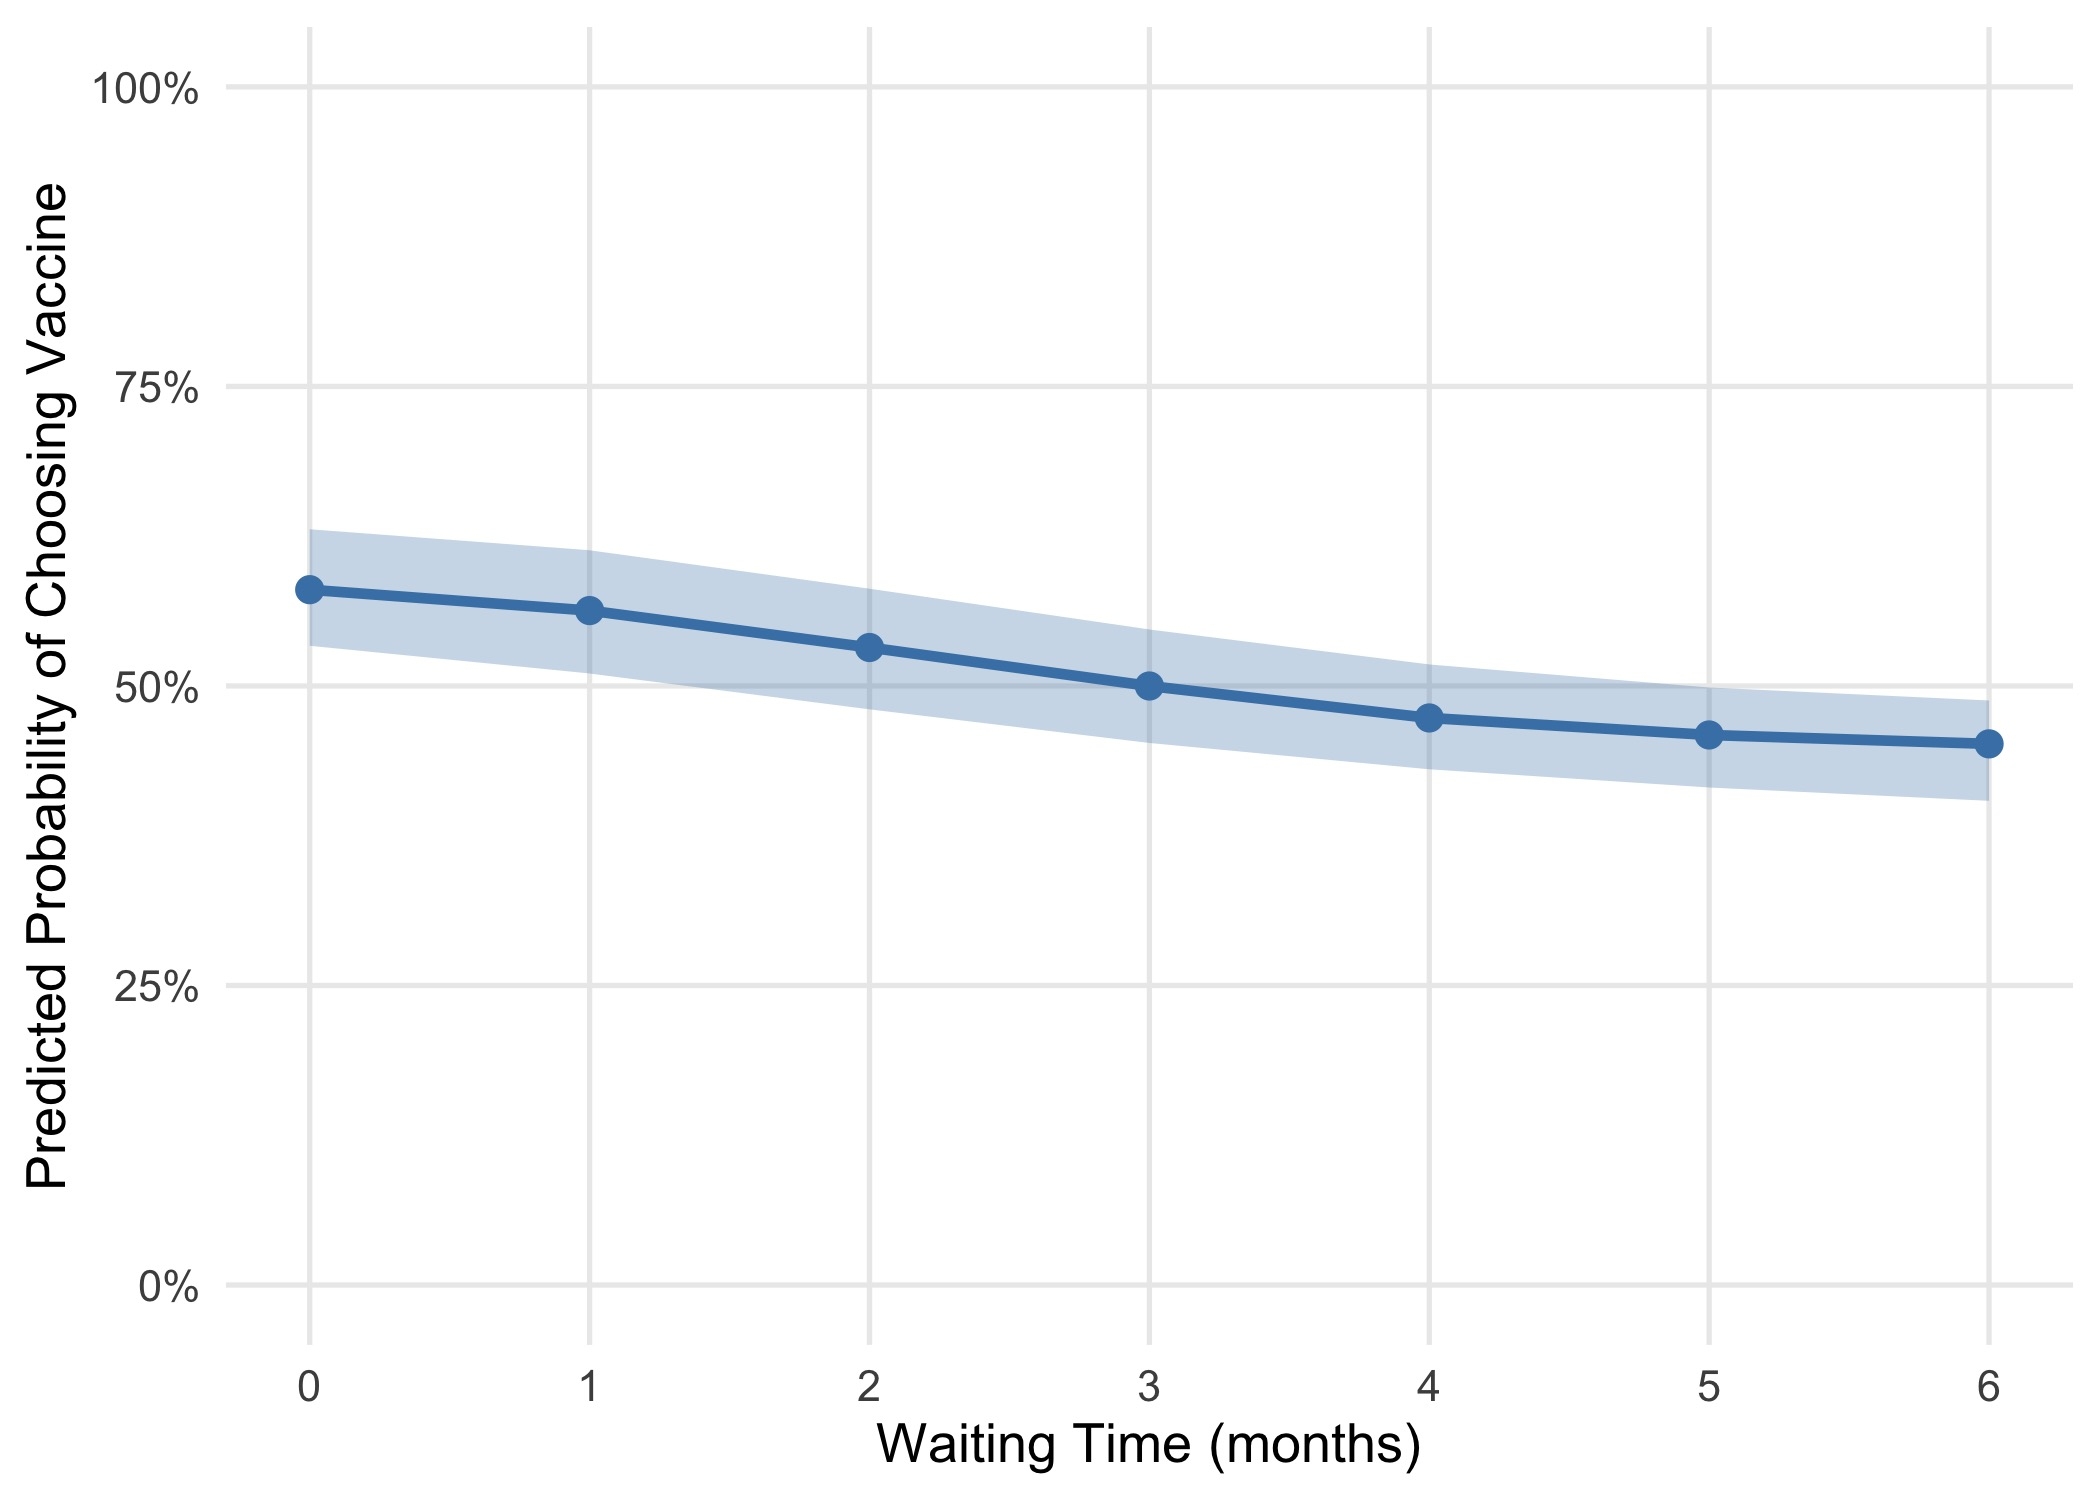
\includegraphics[width=0.8\textwidth]{effect_waiting_time_vaccine_choice.jpg}
\caption{Effect of waiting time on vaccine choice. The figure shows predicted probabilities of selecting the vaccine across different waiting times, with other attributes held at their mean levels. Shaded areas represent 95\% confidence intervals.}
\label{fig:waiting_main}
\end{figure}

\begin{table}[htbp]
\centering
\caption{Main model estimates of vaccine choice (dependent variable: choice)}
\label{tab:main_model}
\begin{tabularx}{\textwidth}{LYYY}
\hline
 & (1) & (2) & (3) \\
 & Conditional Logit & MNL & Mixed Logit \\
\hline
(Intercept): B & & -0.23*** & \\
 & & (0.04) & \\
(Intercept): C & & -0.19* & \\
 & & (0.08) & \\
Waiting time (std) & -0.12*** & -0.10*** & -0.30*** \\
 & (0.02) & (0.02) & (0.03) \\
Vaccine efficacy (std) & 0.15*** & 0.17*** & 0.28*** \\
 & (0.04) & (0.04) & (0.04) \\
Side effects: mild (eff. coding) & -0.13*** & -0.08** & -0.25*** \\
 & (0.03) & (0.03) & (0.03) \\
Side effects: moderate (eff. coding) & 0.35*** & 0.40*** & 0.51*** \\
 & (0.03) & (0.03) & (0.03) \\
Cash incentives (std) & 0.33*** & 0.31*** & 0.42*** \\
 & (0.02) & (0.02) & (0.02) \\
Vaccine origin (domestic) & 0.30*** & 0.29*** & 0.20*** \\
 & (0.04) & (0.04) & (0.05) \\
Opt-out constant & -0.09 & & -0.11 \\
 & (0.08) & & (0.11) \\
SD (waiting time) & & & 1.27*** \\
 & & & (0.08) \\
\hline
AIC & 12,057.90 & 12,015.46 & 10,995.16 \\
BIC & 12,112.67 & 12,078.05 & 11,057.75 \\
Log likelihood & -6,021.95 & -5,999.73 & -5,489.58 \\
Observations & 6,162 & 6,162 & 6,162 \\
\hline
\multicolumn{4}{@{}p{\textwidth}@{}}{Notes: Standard errors in parentheses. *** $p<0.001$, ** $p<0.01$, * $p<0.05$. All models estimated on the full analytic sample ($N=1{,}027$ respondents; 6{,}162 choice observations). Column 1: conditional logit with an opt-out constant. Column 2: multinomial logit with alternative-specific constants (B, C); the opt-out alternative serves as the base category. Column 3: mixed logit with a normally distributed random coefficient on waiting time, 500 Halton draws, and respondent-level panel structure.} \\
\end{tabularx}
\end{table}

\clearpage

\subsection{Heterogeneity in Delay Sensitivity}\label{sec:results_het}

To examine whether the average waiting-time effect masks meaningful heterogeneity across respondents, we characterized the distribution of the random waiting-time coefficient in the mixed logit (Section~\ref{sec:methods}). The estimated standard deviation ($\sigma = 1.440$, SE $= 0.077$) was substantively large relative to the mean ($\beta = -0.425$), implying substantial preference heterogeneity in the magnitude of delay aversion. Under the fitted Normal specification, approximately 38.4\% of the latent coefficient distribution lies above zero. This proportion reflects the assumed symmetric mixing distribution and should not be interpreted as the proportion of respondents who prefer longer delays. Accordingly, the estimated standard deviation provides evidence of substantial heterogeneity, but the shape of that heterogeneity remains distribution-dependent. \textbf{Alternative bounded or asymmetric mixing distributions should be examined in future work.}

We further examined whether waiting-time sensitivity varied systematically across institutional trust groups using subgroup-specific mixed logit models, a categorical interaction specification, and a continuous-interaction specification (estimates reported in the Online Supplementary Material, Appendix~F). The subgroup analysis suggested elevated waiting-time sensitivity among low- and neutral-trust respondents relative to high-trust respondents. In the categorical interaction model (high trust as reference), the joint Wald test of the low-trust and neutral-trust waiting-time interactions was $\chi^2(2) = 13.87$, $p < 0.001$; the neutral-vs-high interaction was individually significant ($z = -3.69$, $p < 0.001$), while the low-vs-high interaction was not ($z = -0.72$, $p = 0.47$). In the continuous-interaction specification, the linear trust-by-waiting interaction was not significant ($p = 0.15$), and adding a quadratic interaction did not improve fit (LR $= 1.21$, $p = 0.27$). The categorical Wald significance is not corroborated by the nested likelihood-ratio test (LR $= 3.95$, $p = 0.14$) nor by the continuous specification test, which assesses a linear-and-quadratic trend across the full five-point trust scale. \textbf{We therefore interpret the apparent trust-related variation as exploratory and hypothesis-generating}; the continuous specification test does not support a robust nonlinear trust-by-waiting mechanism, and the categorical Wald result is most parsimoniously read as driven by the neutral-trust subgroup specifically. Subgroup estimates are reported in the Online Supplementary Material (Appendix~F) for completeness; readers should treat these estimates as descriptive of the present sample rather than as evidence that institutional trust systematically moderates delay sensitivity.

\subsection{Monetary Interpretation of Waiting-Time Burden}

To facilitate interpretation, we converted waiting-time sensitivity into a monetary metric using the trade-off between waiting time and cash incentives estimated from the mixed logit model. Specifically, marginal willingness to accept (MWTA) expresses the amount of compensation respondents would require to tolerate an additional month of waiting. The full-sample estimate indicates that respondents require approximately \textbf{131 RMB per additional month of waiting} (95\% CI computed by the delta method: 111--152 RMB/month; full derivations are reported in the Online Supplementary Material, Section~E). This estimate provides convergent evidence that delay imposes a tangible and nontrivial monetary burden on vaccine choice. MWTA for the trust-specific subgroups is reported in the Online Supplementary Material (Section~E); these subgroup MWTA estimates are interpreted as exploratory given that the continuous specification test did not support a systematic trust-by-waiting interaction.

Across the full sample, respondents required positive monetary compensation to accept additional waiting time, indicating that delay imposed a meaningful perceived burden on vaccine choice. This suggests that reducing waiting time may be especially important for groups facing the highest perceived cost of delay; future studies could examine whether intervention effects vary according to independently measured delay sensitivity rather than relying on post-hoc subgroup partitions.

% elsarticle already handles front-matter pagination; avoid forcing an extra blank page here.

\section{Discussion}\label{sec:discussion}
\doublespacing

This study examines how waiting time influences vaccination decisions. Three main findings emerge. First, longer waiting times reduce the likelihood of stated vaccine choice on average, indicating that delayed protection is associated with reduced stated vaccine choice for many respondents; the mixed logit's Normal specification places roughly 40\% of the coefficient mass above zero, so the negative waiting-time effect is not universal and the magnitude of the effect varies substantially across respondents. Second, the substantial standard deviation of the random waiting-time coefficient indicates substantial preference heterogeneity in the magnitude of delay aversion, although the present data do not identify a discrete typology of respondents. Third, translating delay sensitivity into monetary terms reveals that the perceived cost of waiting is substantial at the population average, but the trust-related variation in this estimate did not survive the continuous specification test and should be treated as exploratory.

\subsection{Delay Sensitivity in Stated Vaccine Choice}

The present findings indicate that waiting time is associated with reduced stated vaccine choice in this sample, with the magnitude of the effect varying substantially across respondents. We interpret these results as evidence of delay sensitivity in stated vaccine choice under a hypothetical epidemic scenario, while acknowledging that the design cannot adjudicate between two non-mutually-exclusive interpretations (see Section~\ref{sec:limitations}): (a) genuine domain-specific delay aversion, where respondents discount delayed protection relative to immediate relief; or (b) rational expectations that a 6-month delay during an epidemic might render the vaccine less necessary as the outbreak subsides. In both readings, longer waiting times are associated with reduced stated vaccine choice; the behavioral-barrier framing reflects interpretation (a) and is presented as the primary reading here, while interpretation (b) is treated as co-equal throughout. Longer waiting times reduced the likelihood of vaccine choice on average---with the magnitude of the effect varying substantially across respondents---indicating that delayed protection carries real perceived cost for many respondents even when other vaccine attributes are held constant. This interpretation is consistent with a broader literature showing that preventive health decisions are shaped not only by expected benefits and risks, but also by the timing and immediacy of those outcomes \citep{AttemaBrouwer2013,AttemaEtAl2018}.

This perspective helps explain why vaccine delay may persist even when vaccination services are available. Waiting does not simply postpone protection; it also imposes immediate inconvenience, prolongs uncertainty, and extends the period during which individuals remain unprotected. In this sense, waiting time may alter how respondents weigh present burdens against future benefits, which is consistent with prior work on present-oriented decision-making and near-term frictions in preventive health behavior \citep{Laibson1997,ODonoghueRabin1999,BrewerEtAl2017,JohnsonEtAl2013}. The findings therefore support the view that delayed access can influence vaccine choice itself, rather than serving only as a neutral logistical feature of program implementation.

More broadly, these results reinforce the importance of service design in preventive health behavior. If even relatively short delays reduce stated willingness to vaccinate, then timeliness should be treated as part of the intervention rather than as a secondary administrative concern. From a behavioral medicine perspective, interventions that reduce waiting time should be tested for effects on actual uptake, because they could act not only by accelerating delivery, but also by lowering the immediate psychological and practical burdens associated with delayed protection.

\subsection{Potential Implications for Intervention Testing}

The preference heterogeneity identified in this study has potential implications for intervention design, but we emphasize that our experiment randomized hypothetical vaccine attributes only; we did not manipulate same-day vaccination, clinician conversation, or other engagement strategies, and we did not validate prospective targeting based on individual delay sensitivity. The results therefore motivate \textit{testing}, not implementation, of specific access-oriented strategies.

Most directly, the strong average disutility for waiting time suggests that same-day or reduced-delay vaccination access is worth testing as a potentially effective lever. In particular, results motivate testing same-day or reduced-delay access in prospective trials, for example by comparing uptake under same-day availability versus scheduled appointments in routine vaccination settings. \textbf{The observed average effect and the substantial random-coefficient standard deviation motivate prospective testing of reduced-delay access; future studies could examine whether intervention effects vary according to independently measured delay sensitivity rather than relying on post-hoc subgroup partitions.}

We likewise caution against interpreting the present heterogeneity evidence as ``clinically actionable subgroups''; the random-coefficient standard deviation indicates that the magnitude of delay aversion varies across respondents, but the present data do not identify discrete subgroups that can be prospectively classified.

\subsection{Discussion of Heterogeneity}

The substantial standard deviation of the random waiting-time coefficient ($\sigma = 1.440$) provides the primary heterogeneity evidence in this study, indicating meaningful variation in the magnitude of delay aversion across respondents. The exploratory subgroup and continuous-interaction analyses on institutional trust provided mixed support for a nonlinear trust-by-waiting pattern, and we treat these findings as hypothesis-generating rather than as evidence of a robust moderation mechanism. \textbf{Trust subgroup analyses (low, neutral, high) and continuous specification tests are reported in the Online Supplementary Material (Appendix~F).}


\subsection{Implications for Preventive Health Delivery and Equity}

The findings have several implications for the design and delivery of preventive health services. First, they suggest that waiting time should be considered a core component of intervention effectiveness rather than a secondary logistical constraint. Even when vaccines are available and acceptable in principle, delays in access can reduce stated vaccine choice by increasing the immediate behavioral burden associated with vaccination \citep{BrewerEtAl2017,LiuEtAl2024}. From this perspective, timely and predictable service delivery may play an important role in shaping preventive health behavior.

Second, the results indicate that the behavioral consequences of waiting time are not evenly distributed across the population. The substantial random-coefficient standard deviation ($\sigma = 1.440$) indicates that waiting-time sensitivity varies substantially across respondents (the Normal specification places roughly 40\% of the latent coefficient mass above zero, so individual-level effect signs are not uniformly negative in the distributional sense), although we did not identify a discrete typology of respondents in this study. Exploratory trust subgroup analyses suggested elevated sensitivity among low- and neutral-trust respondents, but the continuous specification test did not confirm a systematic nonlinear pattern; we therefore interpret trust-related variation as exploratory and hypothesis-generating. \textbf{This suggests that uniform service designs may have unequal effects, with delay-sensitive individuals bearing a disproportionate burden of waiting}. If the patterns we observe in stated preferences translate into actual uptake under real vaccination conditions, they may inform the design of more equitable vaccination strategies.

Third, these findings highlight the importance of designing interventions that address not only vaccine attitudes, but also the timing and predictability of access. Interventions that reduce waiting time, increase scheduling transparency, provide clearer expectations about when protection will be delivered, or strengthen the perceived reliability of service delivery may help mitigate the behavioral burden of delayed protection. In this sense, improving appointment systems, reducing administrative uncertainty, and making delivery timelines more predictable may complement traditional strategies focused on information provision or financial incentives \citep{BrewerEtAl2017,LiuEtAl2024}.

Taken together, the results suggest that improving timeliness and predictability in vaccine delivery may contribute to both higher overall uptake and more equitable outcomes across population groups. From a behavioral medicine perspective, service design features such as waiting time should therefore be treated as integral components of intervention effectiveness rather than as purely operational considerations.

\subsection{Monetary Interpretation of Delay Burden}

Translating waiting-time sensitivity into monetary willingness to accept (MWTA) provides an intuitive interpretation of the behavioral cost of delay. The full-sample estimate indicates that respondents require approximately 131 RMB per additional month of waiting (95\% CI: 80--118), suggesting that delayed protection imposes a tangible and nontrivial burden on vaccine choice.

The full-sample MWTA estimate indicates that respondents required positive monetary compensation to accept additional waiting time, suggesting that delayed protection imposes a tangible burden on vaccine choice at the population average. Exploratory trust subgroup analyses suggested elevated MWTA among neutral-trust respondents, but given that the low versus neutral comparison was not robust across specification choices and the continuous specification did not confirm a systematic pattern, we interpret these differences as exploratory. \emph{Exploratory findings should be tested with pre-registered hypotheses rather than treated as conclusive evidence of a nonlinear mechanism.} Further research is needed to better understand how perceptions of institutional reliability, uncertainty, and service delivery interact to shape responses to delayed protection.

From a policy perspective, these findings suggest that reducing waiting time may be associated with benefits comparable to providing additional incentives. Interventions that shorten delays or improve the predictability of access may therefore yield benefits comparable to financial incentives, while potentially being more scalable and acceptable in public health settings.

\subsection{Comparison with Recent Evidence on Time Preferences and Vaccination}

Our findings contribute to a growing literature examining how time preferences shape vaccination decisions. A recent large-scale study by \cite{Attema2025} investigated present bias and discount rates in COVID-19 vaccination decisions across 22 countries, using choice-list methodology to elicit time preferences separately from vaccination preferences. They found \textbf{no evidence of present bias} (\(\beta \approx 1\), not significantly different from constant discounting) in revealed vaccination preferences, though discount rates varied substantially across countries and vaccination statuses.

Our results appear to diverge from this null finding: we find substantial delay sensitivity in our sample, with waiting time reducing vaccination likelihood to a degree comparable to substantially reducing vaccine effectiveness. Several factors may explain this apparent discrepancy:

\textbf{First, methodological differences.} Attema et al. used choice-list methodology with monetary trade-offs to elicit time preferences separately, then examined their correlation with vaccination status. In contrast, our DCE embedded waiting time directly within the vaccination choice context, capturing trade-offs between delayed protection and other vaccine attributes. The former approach tests whether time preferences \textit{predict} vaccination behavior; the latter tests whether delay sensitivity enters vaccination decisions \textit{directly}.

\textbf{Second, outcome measurement.} Attema et al. analyzed revealed vaccination status (already vaccinated vs. not), which may reflect mandates, availability, and other institutional factors beyond individual preferences. Our stated-preference approach examined hypothetical choices under controlled conditions, isolating the effect of waiting time from confounding factors.

\textbf{Third, population and context.} Our sample was drawn from Wuhan, China, where the pandemic experience and vaccination context differed substantially from the multi-country sample in Attema et al. The high behavioral salience of delayed protection in this setting may amplify delay-sensitive responses relative to contexts where vaccination was already widespread.

\textbf{Reconciling the findings.} These results are not necessarily contradictory. Attema et al.'s null result concerns general time preferences elicited through monetary choices. Our finding of domain-specific delay sensitivity concerns responses to waiting time within vaccination decisions. The discrepancy suggests that delay aversion may be context-dependent, emerging more strongly in the vaccination domain (where delay directly delays protection) than in domain-general monetary trade-offs. Future research should directly compare monetary and health-related delay sensitivity within the same sample to adjudicate between these possibilities.

This interpretation suggests that delay aversion may be context-dependent, emerging more strongly in the vaccination domain (where delay directly delays protection) than in domain-general monetary trade-offs. One candidate mechanism is domain specificity in time preference: Attema and colleagues elicited time preferences using monetary trade-offs, whereas our DCE embeds waiting time directly within the vaccination decision, so that delay is evaluated in the same choice context as protection itself. Prior work in intertemporal choice suggests that health-specific delay framing can activate different evaluation processes than abstract monetary trade-offs, with health-framed delays engaging anticipatory affect and monetary trade-offs engaging abstract valuation \citep{Loewenstein2001,Brewer2017}. We offer this as a tentative mechanism rather than a direct test; the present study is not designed to disentangle these processes, and the question of why vaccine-related delay sensitivity exceeds monetary delay sensitivity remains open. Future research should test this account by comparing domain-specific and domain-general delay elicitation in the same sample. A further consideration concerns the \textit{direction} of Attema et al.'s estimate: their point estimate was $\beta \approx 1$ (constant discounting), but the confidence interval includes values slightly greater than one, which under the standard exponential-discounting parametrization would indicate a very mild \textit{future bias}---a preference for later over earlier outcomes---rather than present bias per se. Their null result on present bias is therefore best read as evidence against strong future-discounting, not against mild directionality in either direction. Whether the vaccine-specific delay sensitivity observed in our DCE would replicate under monetary elicitation tasks in the same sample---or whether the same individuals who exhibit large delay sensitivity in the vaccination choice context would also exhibit present or future bias on a monetary time-preference task---is an open empirical question that the present study does not address. Attema measures domain-general time preferences; our study measures vaccine-context delay sensitivity. Whether the two constructs measure the same underlying disposition, partially overlap, or are distinct remains open. We treat the comparison as descriptive and hypothesis-generating rather than as evidence about the time-preference profile of the Wuhan sample.

\subsection{Limitations}\label{sec:limitations}

\paragraph{Stated Preference and Behavioral Barrier Identification}

We note that discrete choice experiments measure \textit{stated preferences} in hypothetical scenarios, not actual behavior. The extent to which these preferences translate into real-world vaccination decisions depends on external validity conditions that we cannot fully assess \citep{Hensher2015}. This distinction matters for interpreting our ``behavioral barrier'' framing: the observed aversion to delayed vaccination could reflect either (a) genuine delay-sensitive preferences that would manifest in actual behavior, or (b) rational expectations that a 6-month delay during an epidemic might render the vaccine less necessary as the outbreak subsides. Our DCE design did not explicitly distinguish epidemic from endemic framing, limiting our ability to rule out this rational-incidence-decline alternative.

Nevertheless, three considerations support interpreting waiting-time sensitivity as behaviorally meaningful. First, prior DCE studies in vaccination have demonstrated predictive validity for actual uptake \citep{Brown2014,Determann2017}, suggesting that stated preferences capture behaviorally relevant dispositions. Second, the large effect size ($\beta = -0.425$) and substantial MWTA (131 RMB/month) indicate that waiting imposes a perceived cost that would likely influence real decisions, not merely hypothetical inconvenience. Third, the heterogeneity captured by the random-coefficient standard deviation ($\sigma = 1.440$, compared with mean $\beta = -0.425$) suggests that the magnitude of the negative waiting-time effect varies substantially across respondents, consistent with prior work linking stated time preferences to preventive health behavior \citep{Laibson1997}. We therefore interpret findings as evidence that waiting time \textit{operates as} a behavioral barrier whose strength varies substantially across respondents, while acknowledging that behavioral validation through revealed preference studies or experimental interventions would strengthen this claim.

Several limitations should be considered when interpreting these findings. First, the study relies on stated preference data from a discrete choice experiment, which may not fully capture real-world vaccination behavior. Although the design allows for controlled variation in waiting time and other attributes, hypothetical bias cannot be entirely ruled out. \textbf{Hypothetical bias in DCEs} refers to the tendency for respondents to overstate their willingness to accept hypothetical options compared to actual behavior, particularly when decisions involve no real consequences \citep{Murphy2005}. In the context of vaccination, hypothetical bias may manifest as respondents being more willing to tolerate waiting time in a survey setting than they would when facing real scheduling constraints. We attempted to mitigate this bias by using a realistic disease scenario (COVID-like disease), including an opt-out option, and embedding waiting time among other salient vaccine attributes that required genuine trade-offs. Nevertheless, the DCE does not establish the magnitude or direction of hypothetical bias relative to actual vaccination behavior: stated waiting-time sensitivity could in principle overstate or understate real-world responsiveness, and revealed preference studies linking DCE responses to actual vaccination timing would strengthen validity.

A secondary observation is that the population-averaged cash-incentive coefficient is positive and statistically detectable in the mixed logit; we therefore interpret the cash-incentive MWTA derivation as applicable to the full sample. The trust-specific subgroup MWTA estimates, by contrast, are reported as exploratory because the continuous specification test did not support a systematic trust-by-waiting interaction.

Second, the data were collected in Wuhan, China, a city with distinctive pandemic experiences and public-health infrastructure. While the behavioral mechanisms identified are likely to generalize, the magnitude of waiting-time sensitivity and its interaction with institutional trust may differ across populations and health systems. \textbf{Single-city sampling limits geographic representativeness; replication in other Chinese cities or international settings would strengthen external validity.}

Third, the heterogeneity analysis relies on a post-hoc trichotomization of the institutional trust scale. Supplementary analyses using a continuous trust specification with linear and quadratic interaction terms did not confirm a nonlinear relationship (likelihood-ratio test of the quadratic specification, $p = 0.27$). This suggests that the apparent ``neutral trust peak'' may be sensitive to the choice of cutpoints. We therefore interpret the trust-group differences as exploratory findings requiring replication, with the random-coefficient standard deviation providing the primary evidence for population-level heterogeneity in delay aversion. \emph{Exploratory findings should be tested with pre-registered hypotheses rather than treated as conclusive evidence of a nonlinear mechanism.} Further research is needed to better understand how perceptions of institutional reliability, uncertainty, and service delivery interact to shape responses to delayed protection.

Fourth, the heterogeneity evidence based on the random-coefficient standard deviation should be interpreted with appropriate caution regarding model dependence. The fitted Normal distribution places approximately 38.4\% of the latent coefficient mass above zero; this proportion is a property of the distributional assumption rather than a literal estimate of the share of respondents who positively value delay. \textbf{The shape of the heterogeneity distribution is itself model-dependent}, and replication studies with pre-registered hypotheses and larger samples---together with alternative bounded or asymmetric mixing distributions---are needed before the heterogeneity evidence can be used to design targeted interventions.

Finally, while the monetary interpretation of delay provides a useful policy metric, it should be interpreted as an approximation of perceived cost rather than a direct measure of welfare. If the disease were perceived as endemic rather than epidemic, a six-month delay could represent a rational response to low background risk rather than a behavioral barrier, and the waiting-time penalty we estimate may not generalize across epidemic phases. Future work may extend this approach by integrating revealed preference data or experimental interventions.


\subsection{Conclusion}

This study provides exploratory evidence of delay sensitivity in stated vaccine choice among Wuhan adults. Longer delays reduce the likelihood of stated vaccine choice, even when other vaccine attributes remain constant. The substantial random-coefficient standard deviation ($\sigma = 1.440$) indicates meaningful heterogeneity in the magnitude of delay aversion across respondents. \textbf{However, the present data do not identify a discrete typology of respondents.} Exploratory trust subgroup analyses suggested elevated sensitivity among neutral-trust respondents, but the nested categorical interaction likelihood-ratio test did not confirm the interaction (LR $= 3.95$, $p = 0.14$) and the continuous specification test did not support a linear-and-quadratic trend (LR $= 1.21$, $p = 0.27$). \textbf{We therefore interpret the apparent trust-related variation as exploratory and hypothesis-generating; the continuous specification test does not support a robust nonlinear mechanism.} The preference heterogeneity evidence is best summarized by the random-coefficient distribution rather than by a discrete segmentation.

By translating delay sensitivity into monetary terms, the results further demonstrate that waiting time imposes a concrete and unevenly distributed burden on vaccine decision-making. These findings highlight the importance of considering time-related frictions as central components of preventive health interventions.

Overall, improving the timeliness and predictability of vaccine delivery may enhance both uptake and equity. From a behavioral medicine perspective, service design features such as waiting time should therefore be treated not merely as logistical constraints, but as integral determinants of preventive health behavior. The exploratory heterogeneity by institutional trust suggests that the relationship between trust and delay sensitivity warrants further investigation; future research should pre-register hypotheses on theoretically motivated moderators and use continuous specification tests to distinguish genuine moderation from post-hoc cutpoint selection. As discussed in Section~\ref{sec:limitations}, these results are consistent with both genuine delay aversion and rational expectations that a 6-month delay during an epidemic may render the vaccine less necessary; future revealed-preference studies are needed to adjudicate between these accounts.

\section*{Declarations}

\subsection*{Funding}
Not applicable. This research received no specific grant from any funding agency in the public, commercial, or not-for-profit sectors.

\subsection*{Competing Interests}
The authors declare that they have no known competing financial interests or personal relationships that could have appeared to influence the work reported in this paper.

\subsection*{Consent for Publication}
Not applicable. This study reports aggregated survey data with no identifiable individual information.

\subsection*{Code Availability}
Analysis code (R scripts) is available from the corresponding author upon reasonable request.

\subsection*{Author Contributions}
Not applicable for blinded peer review.

\section*{Declaration of Generative AI Use}

Generative artificial intelligence tools were used to assist with language editing, formatting, code and consistency checking, and manuscript critique. All statistical analyses, numerical results, and final scientific interpretations were performed and verified by the authors, who take full responsibility for the content of the manuscript.

\section*{Ethics Approval and Informed Consent}

The study involved anonymous, minimal-risk survey research conducted in China. All study procedures complied with relevant national regulations and institutional guidelines. The study protocol was reviewed by the [BLINDED] Institutional Review Board and determined to be exempt from full board review under Category 2 (survey research with no identifying information). All participants provided informed consent prior to participation.

\section*{Data Availability Statement}

The data that support the findings of this study are not publicly available due to ethical and privacy considerations related to human-subject survey data. De-identified data may be made available from the corresponding author upon reasonable request, subject to approval by the relevant ethics committee.

\clearpage
\begingroup
\singlespacing
\bibliographystyle{plainnat}
\bibliography{references_cleaned}
\endgroup

% ==================== ONLINE SUPPLEMENTARY MATERIAL ====================
\clearpage
\section*{Online Supplementary Material}
\addcontentsline{toc}{section}{Online Supplementary Material}

% Appendix A — Pilot Test
\section*{Appendix A. Pilot Test and Instrument Refinement}
\label{app:A}

This appendix describes the pilot testing procedures used to refine the DCE instrument before full deployment.

\subsection*{A1. Pilot sample}

The instrument was pilot-tested with 60 respondents. Pilot participants completed the full survey instrument, including the DCE choice tasks and demographic questions, and provided open-ended feedback on comprehension and task difficulty.

\subsection*{A2. Feedback collection}

Pilot respondents were asked to:
\begin{itemize}
    \item Paraphrase the meaning of key attributes in their own words
    \item Identify any confusing or ambiguous wording
    \item Report difficulty in making trade-offs between attributes
    \item Suggest improvements to the choice card layout
\end{itemize}

\subsection*{A3. Refinements based on pilot feedback}

Several modifications were made based on pilot responses:
\begin{itemize}
    \item Clarified that waiting time refers to the period before receiving the first dose (not full immunity)
    \item Added visual cues to distinguish between vaccine alternatives
    \item Simplified the wording and presentation of side-effect profiles
    \item Adjusted attribute level ranges based on observed choice patterns
\end{itemize}

\clearpage


% Appendix B — Choice Card
\section*{Appendix B. Choice Card, Design Specification, and Sample Benchmarks}
\label{app:B}

This appendix presents the final DCE card structure, the experimental design specification, and comparisons of the analytic sample with population benchmarks referenced in the main text.

\subsection*{B1. Choice format}

Each task presents two vaccine alternatives and an opt-out. Respondents choose the preferred option for each task.

\subsection*{B2. Core attributes}

The DCE included five attributes:
\begin{itemize}
    \item \textbf{Waiting time to vaccination:} 0, 1, 2, 3, or 6 months
    \item \textbf{Vaccine efficacy:} 50\%, 70\%, or 95\%
    \item \textbf{Side-effect profile:} mild (fatigue 1--2 days), moderate (fever 2 days), or severe (fatigue 1 week)
    \item \textbf{Vaccine origin:} domestic or imported
    \item \textbf{Cash incentive:} 50, 200, or 800 RMB
\end{itemize}

\begin{figure}[H]
    \centering
    \IfFileExists{sample_card.png}{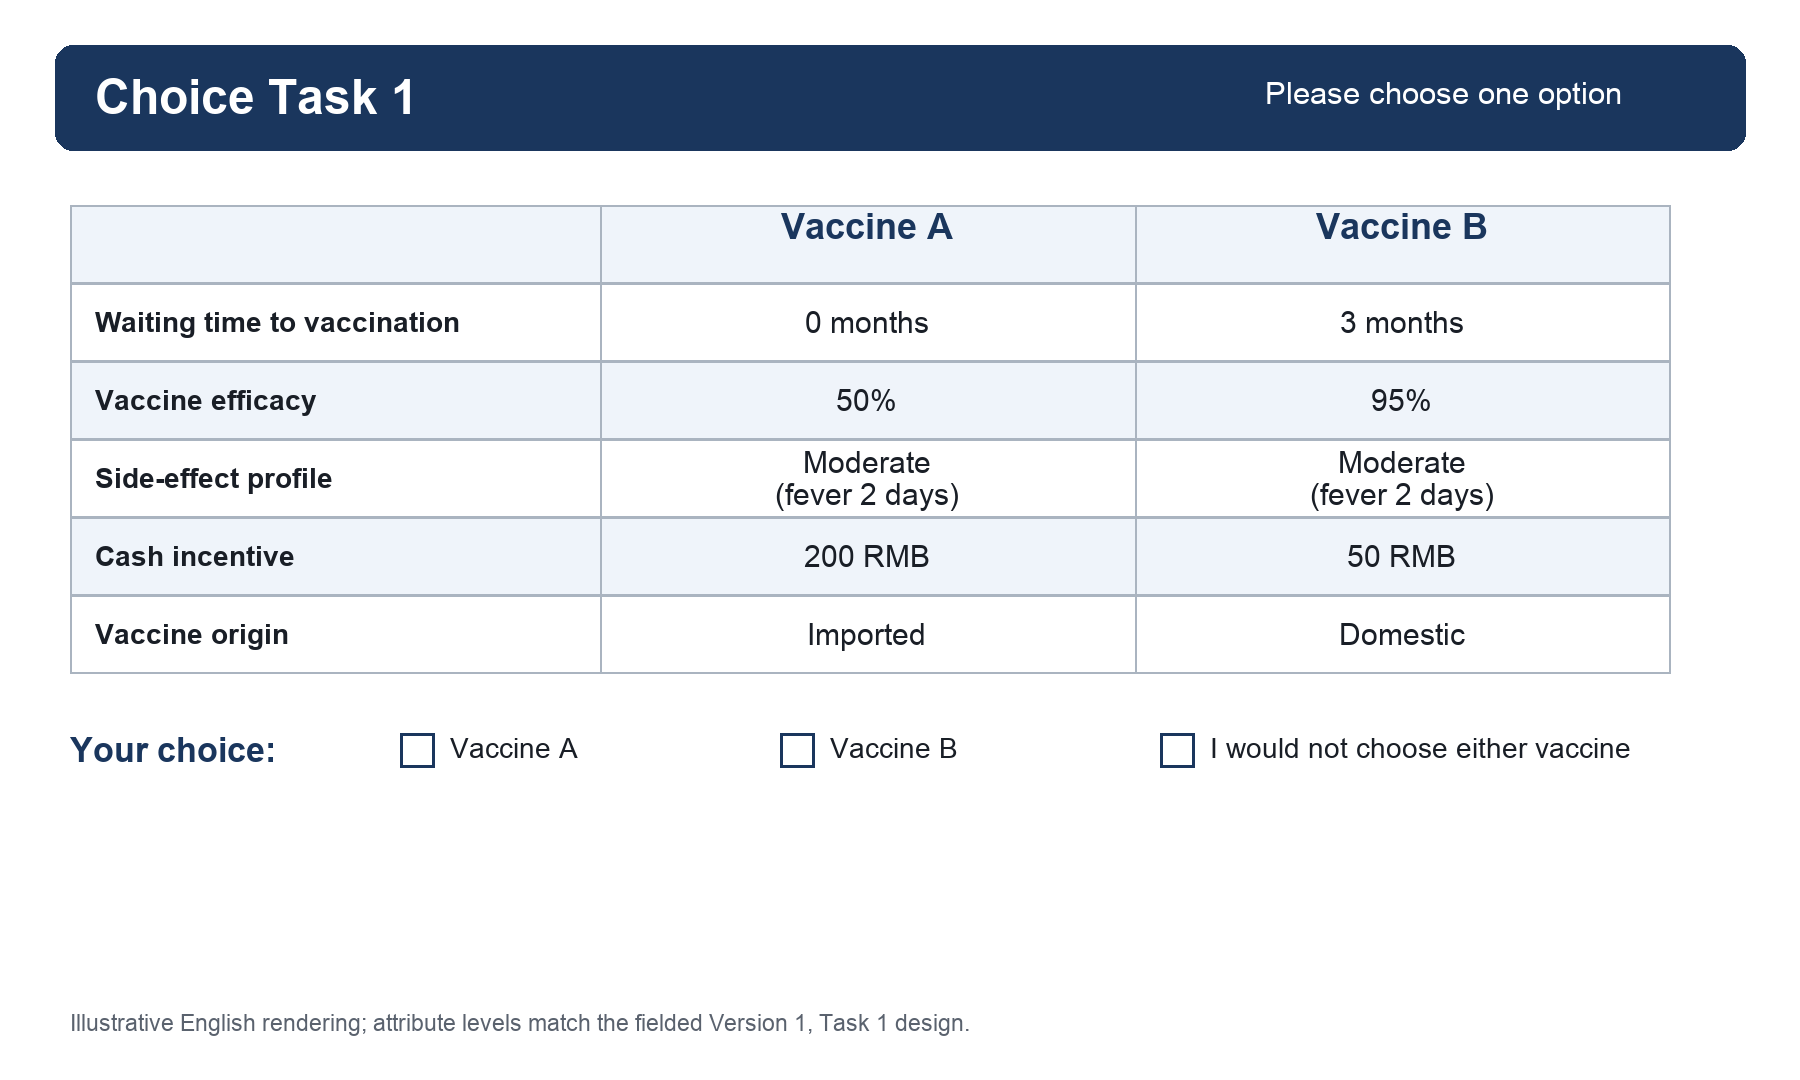
\includegraphics[width=0.9\linewidth]{sample_card.png}}{\fbox{Missing file: sample_card.png}}
    \caption{Final choice card format (illustrative).}
\end{figure}

\subsection*{B3. Experimental design}

The design was generated using the automated design feature of the Wenjuanxing survey platform based on the attribute levels in B2, yielding eight design versions. Every respondent was randomly assigned to one version and completed 6 choice sets (one set per task), each presenting two vaccine profiles (A, B) and an opt-out (``None of these''). Table~\ref{tab:design_versions} reports the number of respondents assigned to each version and the within-version attribute-level balance across the 12 non-opt-out profiles (6 sets $\times$ 2 alternatives). Versions 1--3, which together account for 69.4\% of respondents ($n = 713$), were balanced on efficacy, side-effect profile, cash incentive, and origin, and evenly represented four of the five waiting-time levels (0, 1, 3, and 6 months; the 2-month waiting level appeared only in Version 8); the remaining versions were approximately balanced. Across all eight versions, 85 unique non-opt-out profiles were administered. Fifteen of the 48 choice sets across the eight versions contained a dominated alternative pair; this is relevant to the data-quality screening described in the main text, which treated dominance violations as an inconsistency criterion. The complete 96-row fielded design matrix (8 versions $\times$ 6 tasks × 2 alternatives) is provided as a separate supplementary CSV file (\texttt{Fielded\_DCE\_Design.csv}); this Appendix B reports the version-level summary (Table~\ref{tab:design_versions}) and the complete Version~1 design matrix for illustration (Table~\ref{tab:design_matrix}).

\begin{table}[htbp]
\centering
\caption{DCE design versions: assignment and within-version attribute-level balance (counts out of 12 non-opt-out profiles per version).}
\label{tab:design_versions}
\footnotesize
\begin{tabularx}{\textwidth}{@{}l c Y Y Y Y Y@{}}
\hline
Version & $n$ & Wait 0/1/2/3/6 & Eff 50/70/95 & \shortstack{SE mild/mod/\\severe} & Cash 50/200/800 & \shortstack{Domestic/\\Imported} \\
\hline
1 & 250 & 3/3/0/3/3 & 4/4/4 & 4/4/4 & 4/4/4 & 6/6 \\
2 & 241 & 3/3/0/3/3 & 4/4/4 & 4/4/4 & 4/4/4 & 6/6 \\
3 & 222 & 3/3/0/3/3 & 4/4/4 & 4/4/4 & 4/4/4 & 6/6 \\
4 & 95 & 5/4/0/0/3 & 4/4/4 & 5/6/1 & 6/1/5 & 7/5 \\
5 & 83 & 0/1/0/7/4 & 5/4/3 & 4/4/4 & 3/6/3 & 5/7 \\
6 & 80 & 3/2/0/4/3 & 4/5/3 & 4/3/5 & 3/6/3 & 6/6 \\
7 & 55 & 5/6/0/0/1 & 2/3/7 & 2/2/8 & 4/3/5 & 6/6 \\
8 & 1 & 2/3/1/3/3 & 4/4/4 & 4/4/4 & 4/4/4 & 6/6 \\
\hline
\multicolumn{7}{@{}p{\textwidth}@{}}{\footnotesize \textit{Note.} Counts are within-version frequencies of each level across the 12 non-opt-out profiles. Versions 1--3 are balanced on efficacy, side-effect profile, cash incentive, and origin, and evenly represent four of the five waiting-time levels (0, 1, 3, 6 months); Versions 4--7 deviate from balance (e.g., Version 4 omits the 2- and 3-month levels; Version 7 omits the 2-, 3-, and one of the cash levels). Version 8 is a single-respondent version differing from Version 2 in one profile (waiting time 2 months instead of 0 months); the 2-month waiting level therefore appears only in Version 8.}
\end{tabularx}
\end{table}

The complete design matrix for Version 1 (the largest version, $n = 250$) is:

\begin{table}[H]
\centering
\caption{Complete design matrix for Version 1 ($n=250$ respondents). Opt-out alternative available in every set.}
\label{tab:design_matrix}
\small
\begin{tabular}{clccccc}
\hline
Set & Alt & Waiting time & Efficacy & Side-effect profile & Cash & Origin \\
\hline
1 & A & 0 months & 50\% & Moderate & 200 RMB & Imported \\
1 & B & 3 months & 95\% & Moderate & 50 RMB & Domestic \\
2 & A & 3 months & 70\% & Severe & 50 RMB & Domestic \\
2 & B & 6 months & 50\% & Mild & 800 RMB & Imported \\
3 & A & 1 month & 70\% & Severe & 50 RMB & Domestic \\
3 & B & 1 month & 95\% & Moderate & 200 RMB & Domestic \\
4 & A & 0 months & 50\% & Mild & 800 RMB & Imported \\
4 & B & 6 months & 95\% & Moderate & 200 RMB & Imported \\
5 & A & 6 months & 70\% & Severe & 50 RMB & Domestic \\
5 & B & 3 months & 95\% & Mild & 800 RMB & Domestic \\
6 & A & 0 months & 70\% & Severe & 200 RMB & Imported \\
6 & B & 1 month & 50\% & Mild & 800 RMB & Imported \\
\hline
\end{tabular}
\end{table}

\noindent \textbf{Attribute-level balance (aggregate).} Across all 85 administered non-opt-out profiles, vaccine efficacy (50\%, 70\%, 95\%), side-effect profile (mild, moderate, severe), and cash incentive (50, 200, 800 RMB) each appeared nearly equally often (28--30, 27--30, and 28--29 of 85 profiles, respectively); waiting time appeared in 0, 1, 2, 3, and 6 months with frequencies 22, 22, 1, 20, and 20 (the single 2-month profile occurred in Version 8). Although 0 RMB was specified as a candidate attribute level, it was not represented in any realized version; the administered profiles contained 50, 200, and 800 RMB incentive levels. We therefore do not claim statistical efficiency for this design, and D-error diagnostics are not reported. An earlier archived design export did not correspond to the fielded instrument. The design matrix reported here was therefore reconstructed from the administered respondent-level choice records and verified against the fielded survey; it constitutes the authoritative record of the realized design.

\subsection*{B4. Sample composition and population benchmarks}

The analytic sample ($N = 1{,}027$) was compared with Wuhan adult population benchmarks using 2020 census data. The sample slightly overrepresents respondents with higher educational attainment relative to the Wuhan population. The study does not apply post-stratification weights; unweighted estimates should be interpreted as conditional on the achieved sample composition. Gender and age-group distributions were broadly consistent with population benchmarks after accounting for the sampling quotas.
\clearpage


% Appendix C — Model Estimation
\section*{Appendix C. Model Estimation and Derived Metrics}
\label{app:C}

This appendix summarizes the modeling framework and the derived behavioral metric used in the main analysis.

\subsection*{C1. Utility framework}

For respondent $n$, alternative $j$, and task $t$, the utility of alternative $j$ is:

\[
U_{njt} = V_{njt} + \varepsilon_{njt},
\]

where $\varepsilon_{njt}$ is an i.i.d. type-I extreme-value error term and the systematic component is:

\[
\begin{aligned}
V_{njt} ={}& \beta_{\text{wait},n}\, \text{WaitTime}^{\text{std}}_{jt}
 + \beta_{\text{eff}}\, \text{Efficacy}^{\text{std}}_{jt}
 + \beta_{\text{cash}}\, \text{Cash}^{\text{std}}_{jt} \\
 & + \beta_{\text{se1}}\, \text{SE\_mild}_{jt} + \beta_{\text{se2}}\, \text{SE\_moderate}_{jt}
 + \beta_{\text{origin}}\, \text{Domestic}_{jt}
 + \beta_{\text{opt}}\, \text{ASC\_optout}_{j}.
\end{aligned}
\]

\noindent The coding of each attribute is:

\begin{itemize}
    \item \textbf{Waiting time, efficacy, cash incentive} (continuous): each standardized to mean 0, standard deviation 1 over the full analytic sample before estimation; coefficients are therefore reported in standard-deviation units for these attributes.
    \item \textbf{Side-effect profile} (categorical, three levels): effects-coded with two contrasts. Mild = 1, moderate = 0, severe = $-1$ for the mild contrast; moderate = 1, mild = 0, severe = $-1$ for the moderate contrast. Effects coding is used (rather than dummy coding) so that the omitted category (severe) is assigned $-1$ on both contrasts and the mean utility across the three profiles is centered at zero; the severe-profile utility is recovered as $-(\beta_{\text{se1}} + \beta_{\text{se2}})$.
    \item \textbf{Vaccine origin} (binary): indicator equal to 1 for domestic origin and 0 for imported origin.
    \item \textbf{Opt-out} (alternative-specific constant): $\text{ASC\_optout}_j = 1$ for the opt-out alternative and 0 for vaccine alternatives A and B.
\end{itemize}

\subsection*{C2. Mixed logit estimation}

Preference heterogeneity is modeled via a normally distributed random coefficient on waiting time. The model is estimated by simulated maximum likelihood with 500 Halton draws. Within-respondent correlation across the six choice tasks arises from the random coefficient together with the panel specification of the likelihood: because $\beta_{\text{wait},n}$ is constant across tasks for a given respondent, the joint probability of respondent $n$'s observed sequence of choices is computed by integrating the product of per-task logit probabilities over the mixing distribution,

\[
L_n(\theta) = \int \prod_{t=1}^{6} \left[ \frac{\exp(V_{n c_{nt} t}(\beta_{\text{wait},n}))}{\sum_{j \in J_{nt}} \exp(V_{njt}(\beta_{\text{wait},n}))} \right] \phi(\beta_{\text{wait},n}; \mu_{\text{wait}}, \sigma_{\text{wait}})\, d\beta_{\text{wait},n},
\]

\noindent where $c_{nt}$ is respondent $n$'s chosen alternative in task $t$ and $J_{nt}$ is the choice set (A, B, opt-out). The opt-out alternative is modeled as a fixed alternative-specific constant; this identifies the average opt-out propensity but is not the source of the panel correlation, which comes from the random coefficient and the product-over-tasks likelihood above. Standard errors are clustered at the respondent level.

\subsection*{C3. Derived metric: marginal willingness to accept (MWTA)}

The monthly monetary equivalent of reducing delay is derived from the ratio of the waiting-time coefficient to the cash-incentive coefficient, converting standardized units back to months and RMB. Full derivations and the numerical example are provided in Appendix~E.
\clearpage


% Appendix D — Opt-out Specification
\section*{Appendix D. Opt-out Specification}
\label{app:D}

\subsection*{D1. Opt-out specification in the primary mixed logit}

The primary mixed logit specification models the opt-out alternative as a fixed alternative-specific constant. The opt-out mean coefficient ($\beta = -0.111$, $p = 0.32$) is not statistically distinguishable from zero, indicating no systematic average preference for the opt-out beyond its attribute configuration. The fixed opt-out specification is retained for parsimony and because the focus of the present analysis is the waiting-time coefficient rather than the opt-out utility.




% Appendix E — Trade-off Computation
\section*{Appendix E. Trade-Off Computation and Policy Translation}
\label{app:E}

This appendix reports formulas and examples used to translate waiting-time coefficients into monetary-equivalent policy trade-offs.

\subsection*{E1. MWTA calculation}

The monthly monetary equivalent of reducing delay is computed from the ratio of the waiting-time coefficient to the cash-incentive coefficient, converting standardized units back to months and RMB:

\[
\text{MWTA} = -\frac{\beta_{\text{wait}}}{\beta_{\text{cash}}} \times \frac{\text{SD}_{\text{cash}}}{\text{SD}_{\text{wait}}}
\]

where $\beta_{\text{wait}}$ and $\beta_{\text{cash}}$ are the estimated coefficients on the standardized waiting-time and cash-incentive attributes, and $\text{SD}_{\text{wait}}$ (months) and $\text{SD}_{\text{cash}}$ (RMB) are the sample standard deviations of the raw attribute levels. The ratio $-\beta_{\text{wait}}/\beta_{\text{cash}}$ expresses compensation in standardized cash units per standardized month; multiplying by $\text{SD}_{\text{cash}}/\text{SD}_{\text{wait}}$ converts to RMB per month.

\noindent \textbf{Source of the scaling constants.} The standardization was applied to the full estimation data frame in long format ($N = 18{,}486$ rows: 1{,}027 respondents $\times$ 6 tasks $\times$ 3 alternatives), which includes the opt-out rows. In these rows, waiting time, efficacy, side-effect profile, and cash incentive are coded as structural zeros (the opt-out offers none of the vaccine attributes). The scaling constants are therefore the sample standard deviations computed over all rows: $\text{SD}_{\text{wait}} = 2.206$ months and $\text{SD}_{\text{cash}} = 311.5$ RMB. \textbf{These are the exact scaling constants used to construct the standardized variables in the long-format estimation data, on which all reported models were estimated.}

\subsection*{E2. Full-sample estimate}

Using the mixed logit estimates from the main text ($\beta_{\text{wait}} = -0.425$, $\beta_{\text{cash}} = 0.456$; $\text{SD}_{\text{wait}} = 2.206$ months, $\text{SD}_{\text{cash}} = 311.5$ RMB):

\[
\text{MWTA} = -\frac{-0.425}{0.456} \times \frac{311.5}{2.206} = 0.932 \times 141.2 \approx 132 \text{ RMB/month}
\]

The delta-method 95\% confidence interval is 111--152 RMB/month (delta-method SE: 10 RMB/month). The present study reports MWTA only for the full-sample mixed logit. Trust-specific subgroup MWTA estimates are reported in the next section; these are interpreted as exploratory given that the continuous specification test did not support a systematic trust-by-waiting interaction.

\subsection*{E3. Subgroup monetary equivalents}

For completeness, we report the monthly monetary equivalents (MWTA) computed from the subgroup-specific mixed logit estimates in Appendix~F (400 simulation draws, respondent-level panel). The full-sample estimate is 132 RMB/month; subgroup estimates are 83 RMB/month (high trust), 129 RMB/month (low trust), and 250 RMB/month (neutral trust). These point estimates are descriptive: the continuous trust specification did not support systematic moderation (linear interaction $p = 0.15$; quadratic-vs-linear LR $p = 0.27$), and we do not interpret the subgroup MWTA differences as evidence of systematic trust moderation.

\clearpage


% Appendix F — Trust Subgroup Analysis
\section*{Appendix F. Trust Subgroup Analysis (Supplementary)}
\label{app:F}

This appendix reports the complementary trust subgroup analyses referenced in the main text. These analyses are presented for completeness and comparability with prior literature; they are interpreted as exploratory. The primary heterogeneity evidence in this study is provided by the random waiting-time coefficient in the mixed logit, as reported in the main text.

\subsection*{F1. Trust Subgroup Estimates}

Trust groups were defined by the five-point institutional trust scale (low: $-2$ to $-1$; neutral: $0$; high: $+1$ to $+2$; $n = 226$, $261$, and $446$, respectively). For each group, we estimated a mixed logit model with a normally distributed random coefficient on waiting time (500 Halton draws, respondent-level panel). Table~\ref{tab:trust_subgroup_mwta} reports the waiting-time coefficients and implied MWTA for each subgroup.

\begin{table}[htbp]
\centering
\caption{Trust subgroup mixed logit estimates and implied MWTA}
\label{tab:trust_subgroup_mwta}
\small
\begin{tabular}{lccc}
\hline
 & High trust & Low trust & Neutral trust \\
 & ($n = 446$) & ($n = 226$) & ($n = 261$) \\
\hline
Waiting-time coefficient & $-0.184$ & $-0.292$ & $-0.564$ \\
($SE$) & ($0.039$) & ($0.059$) & ($0.070$) \\
Random-coefficient SD & $1.127$ & $1.287$ & $1.533$ \\
MWTA (RMB/month) & 59 & 101 & 205 \\
\hline
\multicolumn{4}{@{}p{\textwidth}@{}}{\footnotesize \textit{Note.} Subgroup-specific mixed logit models with a normally distributed random coefficient on waiting time (500 Halton draws, respondent-level panel). MWTA converts the waiting-time coefficient to RMB/month using the full-sample scaling constants (see Appendix~E). These point estimates are descriptive; the continuous trust interaction was not statistically significant (Appendix F2), so we do not interpret subgroup differences as evidence of systematic trust moderation.}
\end{tabular}
\end{table}

The point estimates are consistent with the main-text description of elevated delay sensitivity among neutral-trust respondents, and with an intermediate position for low-trust respondents. Given the exploratory nature of these analyses and the multiple-testing context, these subgroup estimates should be interpreted descriptively rather than as confirmatory evidence of discrete group differences.

\subsection*{F2. Categorical and Continuous Interaction Specifications}

We estimated two interaction specifications on the trust-complete subsample ($N = 933$). In the categorical interaction model, high trust was used as the reference category, and interaction terms were added for waiting time with low trust and neutral trust. The joint Wald test of the two interaction coefficients was $\chi^2(2) = 13.87$, $p < 0.001$; the neutral-vs-high interaction was individually significant ($z = -3.69$, $p < 0.001$, coefficient $-0.229$), while the low-vs-high interaction was not ($z = -0.72$, $p = 0.47$, coefficient $-0.045$). A likelihood-ratio comparison against the no-interaction baseline yielded LR $= 3.95$, $p = 0.14$. The Wald and LR results therefore diverge: categorical inference on the trust-by-waiting interaction is test-dependent. The categorical Wald test is significant while the nested LR comparison is not, indicating that the interaction evidence is not robust across specification choices. The substantive driver of the categorical Wald significance is the elevated neutral-vs-high coefficient; the low-vs-high contrast is null.

In the continuous specification, waiting time interacted with the (centered) linear and quadratic trust score. The linear trust-by-waiting interaction was not statistically significant ($p = 0.15$), and adding a quadratic interaction did not improve fit (LR $= 1.21$, $p = 0.27$). The categorical and continuous specifications therefore diverge: the categorical specification detects the elevated neutral-vs-high contrast, while the continuous specification finds no evidence of a linear-or-quadratic trend across the full five-point trust scale. We accordingly treat the subgroup MWTA differences as exploratory, with the neutral-trust point estimate the most descriptively distinctive of the three subgroups but not robustly supported as a general trust-by-waiting mechanism.

\subsection*{F3. Potential mechanisms for future testing}

Several behavioral-medicine frameworks could in principle account for elevated delay sensitivity among lower-trust respondents. First, institutional trust may function as uncertainty reduction: respondents who trust the system may view delays as manageable deviations from a reliable norm, whereas those who do not may be more uncertain whether delayed protection will materialize \citep{Hardin2002}. Second, motivated processing accounts suggest that high-trust respondents minimize the perceived burden of waiting, while lower-trust respondents may disengage from the institutional offer or process delay more ``coldly'' \citep{Kahan2013,Betsch2017}. Third, reference-dependent evaluation predicts that respondents without a clear reference point for institutional delivery experience each additional month of delay as a novel loss \citep{Kahneman1979,Tversky1992}. These accounts are not mutually exclusive, and the current data do not discriminate among them; they are offered as candidate explanations for future experimental testing (e.g., manipulating institutional-reliability framing or reference points).

\subsection*{F4. Interpretation and Limitations}

The trust-group findings are exploratory and hypothesis-generating rather than conclusive: the point estimates are descriptively consistent with a ``neutral peak'' in delay sensitivity, but the continuous specification test did not confirm a systematic nonlinear relationship. We therefore do not interpret the subgroup MWTA differences or the candidate mechanisms as established; the random-coefficient standard deviation provides the primary evidence for population-level heterogeneity.
\clearpage



\end{document}
